%---------- Inleiding ---------------------------------------------------------

% TODO: Is dit voorstel gebaseerd op een paper van Research Methods die je
% vorig jaar hebt ingediend? Heb je daarbij eventueel samengewerkt met een
% andere student?
% Zo ja, haal dan de tekst hieronder uit commentaar en pas aan.

%\paragraph{Opmerking}

% Dit voorstel is gebaseerd op het onderzoeksvoorstel dat werd geschreven in het
% kader van het vak Research Methods dat ik (vorig/dit) academiejaar heb
% uitgewerkt (met medesturent VOORNAAM NAAM als mede-auteur).
% 

\section{Inleiding}%
\label{sec:inleiding}

%Waarover zal je bachelorproef gaan? Introduceer het thema en zorg dat volgende zaken zeker duidelijk aanwezig zijn:

%\begin{itemize}
%  \item kaderen thema
%  \item de doelgroep
%  \item de probleemstelling en (centrale) onderzoeksvraag
%  \item de onderzoeksdoelstelling
%\end{itemize}

%Denk er aan: een typische bachelorproef is \textit{toegepast onderzoek}, wat betekent dat je start vanuit een concrete probleemsituatie in bedrijfscontext, een \textbf{casus}. Het is belangrijk om je onderwerp goed af te bakenen: je gaat voor die \textit{ene specifieke probleemsituatie} op zoek naar een goede oplossing, op basis van de huidige kennis in het vakgebied.

%De doelgroep moet ook concreet en duidelijk zijn, dus geen algemene of vaag gedefinieerde groepen zoals \emph{bedrijven}, \emph{developers}, \emph{Vlamingen}, enz. Je richt je in elk geval op it-professionals, een bachelorproef is geen populariserende tekst. Eén specifiek bedrijf (die te maken hebben met een concrete probleemsituatie) is dus beter dan \emph{bedrijven} in het algemeen.

%Formuleer duidelijk de onderzoeksvraag! De begeleiders lezen nog steeds te veel voorstellen waarin we geen onderzoeksvraag terugvinden.

%Schrijf ook iets over de doelstelling. Wat zie je als het concrete eindresultaat van je onderzoek, naast de uitgeschreven scriptie? Is het een proof-of-concept, een rapport met aanbevelingen, \ldots Met welk eindresultaat kan je je bachelorproef als een succes beschouwen?

In de hedendaagse digitale wereld spelen digitale bestanden een grote rol, zowel in privé- als in bedrijfscontext \autocite{MaritimeSurvey2022}. Documenten, onderzoeksgegevens en administratieve dossiers worden digitaal opgemaakt, bijgehouden en wereldwijd verspreid. Papieren documenten en boeken worden gedigitaliseerd om ze eenvoudig te verspreiden en te raadplegen. Hoewel dit het voor particulieren en bedrijven gemakkelijker maakt om een eigen bibliotheek aan informatie bij te houden, brengt dit ook complicaties met zich mee.

De grootste hiervan is toegankelijkheid. Wat gebeurt er wanneer men zich in een gebied bevindt zonder betrouwbare verbinding met het globale netwerk? Wat gebeurt er tijdens rampen, wanneer de infrastructuur wordt weggevaagd door tsunamis of aardbevingen \autocite{WinlinkEmcomm}? Wat zijn de beperkingen op zee, waar connectiviteit structureel onbetrouwbaar is \autocite{MaritimeSurvey2022}?

Hoewel er reeds oplossingen bestaan zoals Starlink en OneWeb, zijn deze voor particulieren en kleine bedrijven vaak financieel of praktisch ontoereikend. De alternatieven voor deze doelgroep zijn onvoldoende onderzocht. Bestaande draadloze communicatietechnologieën, zoals radioverbindingen, bieden potentieel een haalbaar alternatief, maar de toepasbaarheid ervan voor bestandsoverdracht op afstand is nog niet grondig in kaart gebracht.

\subsection*{Probleemstelling}

De centrale onderzoeksvraag luidt:

\begin{quote}
  \textit{Hoe kan een verbinding worden opgezet met een eigen fileserver via een radioverbinding, en wat zijn de technische randvoorwaarden en maximale afstandsbeperkingen voor een werkende implementatie?}
\end{quote}

Bijkomende deelvragen die het onderzoek structureren, zijn:

\begin{itemize}
  \item Welke radioprotocollen (zoals AX.25, Winlink, of IP-over-radio) zijn geschikt voor bestandsoverdracht, en wat zijn hun kenmerken op het vlak van bandbreedte, betrouwbaarheid en bereik?
  \item Welke multiplexingtechnieken — zoals \textit{frequency division multiplexing} (FDM) en \textit{time division multiplexing} (TDM) — zijn van toepassing binnen radiogebaseerde datacommunicatie, en welke beperkingen leggen zij op?
  \item Wat is de maximale praktische afstand waarover een bestandsoverdracht via radioverbinding haalbaar is, afhankelijk van frequentieband en omgevingsfactoren?
  \item Welke infrastructuur en configuratie zijn minimaal vereist voor een werkend proof-of-concept?
\end{itemize}

\subsection*{Doelgroep}

Dit onderzoek richt zich op IT-professionals en netwerkingenieurs die actief zijn in omgevingen met beperkte of onbetrouwbare internetconnectiviteit — zoals maritieme operatoren, hulpverleningsorganisaties in rampgebieden, of bedrijven in afgelegen regio's. De inzichten zijn tevens relevant voor radiocommunicatiespecialisten die netwerktoepassingen willen integreren in bestaande radioinfrastructuur.

\subsection*{Onderzoeksdoelstelling en methodologie}

Het doel van dit onderzoek is na te gaan of en hoe een fileserver bereikbaar gemaakt kan worden via een radioverbinding, met aandacht voor de technische haalbaarheid, de vereiste protocollen en de praktische beperkingen zoals maximale afstand en doorvoersnelheid.

De gehanteerde onderzoeksmethode omvat drie fasen:

\begin{enumerate}
  \item \textbf{Literatuurstudie:} Een grondige verkenning van relevante radioprotocollen (AX.25, Winlink, IP-over-radio), netwerktopologieën voor draadloze communicatie, en multiplexingtechnieken (FDM, TDM). Tevens worden de fysische eigenschappen van radiogolven bestudeerd, waaronder de invloed van frequentieband op bereik en datadoorvoer \autocite{Tanenbaum2021}.
  \item \textbf{Vergelijkende analyse:} De geïdentificeerde protocollen en technieken worden vergeleken op criteria zoals maximale afstand, bandbreedte, hardwarevereisten en complexiteit van implementatie.
  \item \textbf{Proof-of-concept:} Op basis van de analyse wordt een minimale werkende opstelling gebouwd en getest, bestaande uit een radiozender/-ontvanger en een fileserver, om de theoretische bevindingen empirisch te valideren.
\end{enumerate}

Het onderzoek kan drie mogelijke uitkomsten opleveren:

\begin{itemize}
  \item Een werkend proof-of-concept dat aantoont hoe een fileserver via radioverbinding bereikbaar gemaakt kan worden.
  \item Een theoretisch onderbouwde oplossingsarchitectuur die de implementatie mogelijk maakt, indien een volledig werkende opstelling buiten bereik valt.
  \item De gemotiveerde uitsluiting van radioverbindingen als haalbare oplossing voor dit probleem, op basis van vastgestelde technische beperkingen.
\end{itemize}

Naast het beantwoorden van de onderzoeksvraag beoogt dit onderzoek een basis te vormen voor verdere technologische ontwikkelingen en vervolgonderzoek binnen het domein van radiogebaseerde datacommunicatie.
%---------- Stand van zaken ---------------------------------------------------

\section{Literatuurstudie}%
\label{sec:literatuurstudie}

% Hier beschrijf je de \emph{state-of-the-art} rondom je gekozen onderzoeksdomein, d.w.z.\ een inleidende, doorlopende tekst over het onderzoeksdomein van je bachelorproef. Je steunt daarbij heel sterk op de professionele \emph{vakliteratuur}, en niet zozeer op populariserende teksten voor een breed publiek. Wat is de huidige stand van zaken in dit domein, en wat zijn nog eventuele open vragen (die misschien de aanleiding waren tot je onderzoeksvraag!)?

% Je mag de titel van deze sectie ook aanpassen (literatuurstudie, stand van zaken, enz.). Zijn er al gelijkaardige onderzoeken gevoerd? Wat concluderen ze? Wat is het verschil met jouw onderzoek?

% Verwijs bij elke introductie van een term of bewering over het domein naar de vakliteratuur, bijvoorbeeld~\autocite{Hykes2013}! Denk zeker goed na welke werken je refereert en waarom.

% Draag zorg voor correcte literatuurverwijzingen! Een bronvermelding hoort thuis \emph{binnen} de zin waar je je op die bron baseert, dus niet er buiten! Maak meteen een verwijzing als je gebruik maakt van een bron. Doe dit dus \emph{niet} aan het einde van een lange paragraaf. Baseer nooit teveel aansluitende tekst op eenzelfde bron.

% Als je informatie over bronnen verzamelt in JabRef, zorg er dan voor dat alle nodige info aanwezig is om de bron terug te vinden (zoals uitvoerig besproken in de lessen Research Methods).

% Voor literatuurverwijzingen zijn er twee belangrijke commando's:
% \autocite{KEY} => (Auteur, jaartal) Gebruik dit als de naam van de auteur
%   geen onderdeel is van de zin.
% \textcite{KEY} => Auteur (jaartal)  Gebruik dit als de auteursnaam wel een
%   functie heeft in de zin (bv. ``Uit onderzoek door Doll & Hill (1954) bleek
%   ...'')

% Je mag deze sectie nog verder onderverdelen in subsecties als dit de structuur van de tekst kan verduidelijken.

In deze literatuurstudie wordt de huidige stand van zaken binnen radiogebaseerde communicatie onderzocht, met nadruk op mogelijke oplossingen voor het zenden en ontvangen van digitale bestanden. Het doel is een conceptueel kader te schetsen dat als theoretische onderbouwing dient voor dit onderzoek.

\subsection{Connectiviteit in afgelegen gebieden en noodsituaties}

Toegang tot digitale bestanden is in de hedendaagse samenleving essentieel \autocite{MaritimeSurvey2022}, maar blijft in uiteenlopende situaties een uitdaging. Satellietnetwerken zoals Starlink en OneWeb bieden weliswaar globale dekking, maar kampen met hoge abonnementskosten, aanzienlijke latency en beperkte toegankelijkheid voor particulieren en kleine bedrijven \autocite{MaritimeSurvey2022}. In noodsituaties waarbij de bestaande infrastructuur is uitgevallen, blijft robuuste digitale communicatie bovendien een kritieke behoefte \autocite{WinlinkEmcomm}.

Deze beperkingen tonen aan dat er behoefte is aan alternatieve methoden die onafhankelijk zijn van een centrale infrastructuur, maar toch voldoende capaciteit kunnen garanderen voor het raadplegen van digitale bestanden.

\subsection{Radiofrequenties en signaalpropagatie}

Radiogebaseerde communicatie maakt gebruik van elektromagnetische golven die zich door de lucht voortplanten. De keuze van frequentieband heeft een directe invloed op zowel het maximale bereik als de beschikbare bandbreedte \autocite{Tanenbaum2021}. Lagere frequenties, zoals HF-banden (3--30 MHz), kunnen grote afstanden overbruggen via reflecties op de ionosfeer, maar bieden slechts een beperkte doorvoersnelheid. Hogere frequenties, zoals de VHF- (30--300 MHz) en UHF-banden (300 MHz--3 GHz), laten hogere datasnelheden toe, maar hebben een kleiner bereik en vereisen doorgaans een vrije zichtlijn tussen zender en ontvanger \autocite{Tanenbaum2021}.

De maximale praktische afstand van een radioverbinding wordt bepaald door een combinatie van factoren: zendvermogen, antenneversterking, frequentieband, terreinprofiel en atmosferische omstandigheden. Voor microwave point-to-point verbindingen in de GHz-range geldt een typisch operationeel bereik van enkele tientallen kilometers, mits er sprake is van \textit{line of sight} \autocite{MicrowavePtP5G}.

\subsection{Multiplextechnieken in radiogebaseerde datacommunicatie}

Om meerdere signalen efficiënt over een gedeeld radiokanaal te transporteren, worden multiplextechnieken toegepast \autocite{Tanenbaum2021}. De twee meest voorkomende zijn:

\begin{itemize}
  \item \textbf{Frequency Division Multiplexing (FDM):} Het beschikbare frequentiespectrum wordt opgedeeld in meerdere subbanden, elk toegewezen aan een afzonderlijk kanaal. Signalen worden gelijktijdig verzonden zonder elkaar te storen, op voorwaarde dat de subbanden voldoende van elkaar gescheiden zijn. FDM wordt veel gebruikt in analoge en digitale radiosystemen, waaronder FM-radio en 4G/LTE \autocite{Tanenbaum2021}.
  \item \textbf{Time Division Multiplexing (TDM):} Meerdere signalen maken gebruik van hetzelfde frequentiekanaal, maar worden afwisselend verzonden in vaste tijdsloten. TDM vereist nauwkeurige tijdssynchronisatie tussen zender en ontvanger, maar laat een efficiënter gebruik van de beschikbare bandbreedte toe wanneer niet alle kanalen continu actief zijn \autocite{Tanenbaum2021}.
\end{itemize}

In de praktijk worden deze technieken gecombineerd: moderne systemen zoals OFDM (\textit{Orthogonal Frequency Division Multiplexing}) integreren elementen van beide benaderingen en vormen de basis van hedendaagse draadloze standaarden \autocite{Tanenbaum2021}.

\subsection{Protocollen voor radiogebaseerde dataoverdracht}

Binnen de amateurradio-gemeenschap bestaan reeds systemen voor dataoverdracht via radiogolven. Een veelgebruikt protocol op de datalinklaag is AX.25, een pakketradioprotocol dat is afgeleid van het X.25-standaard en specifiek is ontworpen voor amateurradiocommunicatie \autocite{Tanenbaum2021}. AX.25 biedt foutdetectie en beperkte foutcorrectie, maar kent een lage doorvoersnelheid die het minder geschikt maakt voor grote bestandsoverdrachten.

Bovenop dergelijke protocollen zijn bredere systemen gebouwd, waarvan Winlink het meest gekende voorbeeld is. Winlink is een wereldwijd netwerk dat gebruikmaakt van HF-, VHF- en UHF-radiofrequenties om e-mailcommunicatie mogelijk te maken \autocite{WinlinkOverview}. Het wordt beschreven als een hybride radiosysteem, ontworpen voor communicatie in afgelegen gebieden en in noodsituaties \autocite{WinlinkEmcomm, WinlinkHybrid}. Hoewel Winlink beperkte bijlagen ondersteunt, is het primair ontworpen voor berichtuitwisseling en daarmee ontoereikend als volwaardige oplossing voor toegang tot een fileserver.

Een verdere optie is IP-over-radio: het tunnelen van standaard IP-verkeer over een radioverbinding, waardoor bestaande netwerktoepassingen — waaronder bestandsoverdrachten via protocollen zoals FTP of SMB — in principe over een radiokanaal kunnen worden aangeboden \autocite{Tanenbaum2021}. Dit concept vormt de theoretische basis voor de in dit onderzoek voorgestelde opstelling.

\subsection{Straalverbindingen als proof-of-concept}

Voor dit onderzoek wordt gefocust op straalverbindingen (\textit{point-to-point wireless links}), waarbij twee antennes rechtstreeks op elkaar gericht zijn. Deze opstelling biedt een grotere bandbreedte dan ionosferische propagatie \autocite{WirelessBackhaulSurvey, MicrowavePtP5G}, maar vereist een vrije zichtlijn (\textit{line of sight}) tussen beide antennes \autocite{MicrowavePtP5G}. In de praktijk worden dergelijke verbindingen al op grote schaal ingezet als draadloze backhaul in telecomnetwerken \autocite{WirelessBackhaulSurvey}.

De keuze voor een straalverbinding als proof-of-concept is verantwoord omdat dezelfde technologie en protocollen worden gebruikt als in grootschalige toepassingen, waardoor de resultaten overdraagbaar zijn naar bredere implementaties \autocite{WirelessBackhaulSurvey}.

\subsection{Lacunes in de bestaande kennis}

Hoewel diverse technologieën bestaan voor radiogebaseerde communicatie \autocite{MaritimeSurvey2022}, bespreekt geen van de onderzochte bronnen het gebruik ervan om toegang te bieden tot een persoonlijke fileserver. De bestaande literatuur richt zich voornamelijk op noodcommunicatie \autocite{WinlinkEmcomm}, professionele backhaul \autocite{MicrowavePtP5G, WirelessBackhaulSurvey} of beperkte diensten zoals e-mail \autocite{WinlinkOverview}. Dit onderzoek richt zich op de ontbrekende verbinding tussen deze deeldomeinen: de technische haalbaarheid van persoonlijke bestandstoegang via een zelfopgezette radioverbinding.

%---------- Methodologie ------------------------------------------------------
\section{Methodologie}%
\label{sec:methodologie}

%Hier beschrijf je hoe je van plan bent het onderzoek te voeren. Welke onderzoekstechniek ga je toepassen om elk van je onderzoeksvragen te beantwoorden? Gebruik je hiervoor literatuurstudie, interviews met belanghebbenden (bv.~voor requirements-analyse), experimenten, simulaties, vergelijkende studie, risico-analyse, PoC, \ldots?

%Valt je onderwerp onder één van de typische soorten bachelorproeven die besproken zijn in de lessen Research Methods (bv.\ vergelijkende studie of risico-analyse)? Zorg er dan ook voor dat we duidelijk de verschillende stappen terug vinden die we verwachten in dit soort onderzoek!

%Vermijd onderzoekstechnieken die geen objectieve, meetbare resultaten kunnen opleveren. Enquêtes, bijvoorbeeld, zijn voor een bachelorproef informatica meestal \textbf{niet geschikt}. De antwoorden zijn eerder meningen dan feiten en in de praktijk blijkt het ook bijzonder moeilijk om voldoende respondenten te vinden. Studenten die een enquête willen voeren, hebben meestal ook geen goede definitie van de populatie, waardoor ook niet kan aangetoond worden dat eventuele resultaten representatief zijn.

%Uit dit onderdeel moet duidelijk naar voor komen dat je bachelorproef ook technisch voldoen\-de diepgang zal bevatten. Het zou niet kloppen als een bachelorproef informatica ook door bv.\ een student marketing zou kunnen uitgevoerd worden.

%Je beschrijft ook al welke tools (hardware, software, diensten, \ldots) je denkt hiervoor te gebruiken of te ontwikkelen.

%Probeer ook een tijdschatting te maken. Hoe lang zal je met elke fase van je onderzoek bezig zijn en wat zijn de concrete \emph{deliverables} in elke fase?

Dit onderzoek hanteert een experimenteel-technische aanpak om te bepalen of een betrouwbare verbinding met een eigen fileserver via een radioverbinding haalbaar is. Het onderzoek is opgebouwd uit vier opeenvolgende fasen, elk met concrete deliverables en een geschatte doorlooptijd.

\subsection{Fase 1: Literatuurstudie}

In de eerste fase wordt de vakliteratuur rond radiogebaseerde dataoverdracht, straalverbindingen en fileserverprotocollen systematisch in kaart gebracht. Concreet komen de volgende onderwerpen aan bod:

\begin{itemize}
  \item Eigenschappen en beperkingen van radiofrequentiebanden (HF, VHF, UHF, microwave) met betrekking tot bandbreedte en maximaal bereik.
  \item Dataprotocollen voor radioverbindingen: AX.25, IP-over-radio en Winlink.
  \item Multiplextechnieken (FDM, TDM) en hun impact op doorvoersnelheid en kanaalbezetting.
  \item Wettelijke beperkingen voor radioamateurbanden in België (BIPT-regelgeving).
  \item Bestandsoverdrachtsprotocollen (FTP, SMB, SCP) en hun vereisten op netwerkniveau.
\end{itemize}

\textbf{Deliverable:} Een uitgewerkte literatuurstudie met een theoretisch kader en een overzicht van technische randvoorwaarden.

\subsection{Fase 2: Requirementsanalyse}

Op basis van de literatuurstudie worden meetbare functionele en niet-functionele eisen opgesteld waaraan de proefopstelling moet voldoen. Deze requirements omvatten onder meer:

\begin{itemize}
  \item \textbf{Minimale bandbreedte:} voldoende doorvoersnelheid voor het ophalen van bestanden binnen een aanvaardbare tijdsspanne.
  \item \textbf{Maximale latency:} de verbindingsvertraging mag de werking van het gekozen bestandsoverdrachtsprotocol niet verstoren.
  \item \textbf{Verbindingsstabiliteit:} maximaal aanvaardbaar packet loss percentage tijdens een overdracht.
  \item \textbf{Wettelijke conformiteit:} de gebruikte frequenties en zendvermogens voldoen aan de Belgische radioamateurregelgeving.
  \item \textbf{Maximale afstand:} de beoogde afstand tussen zender en ontvanger, bepaald op basis van de gekozen frequentieband en antenneconfiguratie.
\end{itemize}

\textbf{Deliverable:} Een gestructureerd requirements-document dat als toetsingskader dient voor de evaluatie van de proof-of-concept.

\subsection{Fase 3: Proof-of-Concept}

In de derde fase wordt een minimale werkende opstelling gebouwd en getest. De hardware bestaat uit twee computers — één geconfigureerd als fileserver, één als client — verbonden via een punt-tot-punt straalantenne-opstelling. De volgende stappen worden doorlopen:

\begin{enumerate}
  \item \textbf{Hardwareselectie en -configuratie:} keuze van geschikte straalantennes, radiohardware (zoals SDR-modules of dedicated radiomodems) en bekabeling op basis van de requirements.
  \item \textbf{Netwerklaagconfiguratie:} opzetten van IP-over-radio of een equivalent protocol zodat standaard TCP/IP-verkeer over de radioverbinding kan worden gerouteerd.
  \item \textbf{Fileserverconfiguratie:} installatie en configuratie van een fileserverdienst (bv. een FTP- of SFTP-server) op de servernode.
  \item \textbf{Testoverdrachten:} uitvoeren van gecontroleerde bestandsoverdrachten van variërende bestandsgroottes om de prestaties te meten.
\end{enumerate}

Tijdens de testfase worden de volgende metrieken geregistreerd:

\begin{itemize}
  \item Gemeten bandbreedte (Mbit/s of Kbit/s) bij verschillende bestandsgroottes.
  \item Packet loss percentage via \texttt{ping} en \texttt{iperf}.
  \item Bestandsoverdrachttijden voor een representatieve set testbestanden.
  \item Verbindingsstabiliteit over een langere meetperiode.
\end{itemize}

\textbf{Gebruikte tools:} Linux (serveromgeving), \texttt{iperf3} (bandbreedtemeting), \texttt{vsftpd} of \texttt{OpenSSH} (fileserverdienst).

\textbf{Deliverable:} Een werkende proof-of-concept opstelling met gedocumenteerde meetresultaten, of een onderbouwde technische verklaring waarom een werkende opstelling niet haalbaar bleek.

\subsection{Fase 4: Evaluatie en conclusie}

In de laatste fase worden de meetresultaten uit de proof-of-concept getoetst aan de requirements die in fase 2 zijn opgesteld. Per requirement wordt bepaald of aan de gestelde eis is voldaan. Op basis van deze analyse wordt een eindconclusie geformuleerd over de technische haalbaarheid van radiogebaseerde toegang tot een persoonlijke fileserver.

Indien de proof-of-concept niet volledig slaagt, worden de vastgestelde knelpunten gedocumenteerd en worden aanbevelingen geformuleerd voor vervolgonderzoek of alternatieve benaderingen.

\textbf{Deliverable:} Een evaluatierapport met een haalbaarheidsoordeel, een overzicht van de bereikte en niet-bereikte requirements, en aanbevelingen voor verdere ontwikkeling.
%---------- Verwachte resultaten ----------------------------------------------
\section{Verwacht resultaat, conclusie}%
\label{sec:verwachte_resultaten}

% Hier beschrijf je welke resultaten je verwacht. Als je metingen en simulaties uitvoert, kan je hier al mock-ups maken van de grafieken samen met de verwachte conclusies. Benoem zeker al je assen en de onderdelen van de grafiek die je gaat gebruiken. Dit zorgt ervoor dat je concreet weet welk soort data je moet verzamelen en hoe je die moet meten.

% Wat heeft de doelgroep van je onderzoek aan het resultaat? Op welke manier zorgt jouw bachelorproef voor een meerwaarde?

% Hier beschrijf je wat je verwacht uit je onderzoek, met de motivatie waarom. Het is \textbf{niet} erg indien uit je onderzoek andere resultaten en conclusies vloeien dan dat je hier beschrijft: het is dan juist interessant om te onderzoeken waarom jouw hypothesen niet overeenkomen met de resultaten.

Op basis van de literatuurstudie en de geformuleerde onderzoeksvraag worden de volgende resultaten verwacht.

\subsection{Technische haalbaarheid}

Gezien de bestaande toepassingen van punt-tot-punt straalverbindingen in professionele backhaul-omgevingen \autocite{WirelessBackhaulSurvey, MicrowavePtP5G}, is de verwachting dat een radioverbinding met voldoende bandbreedte voor bestandsoverdracht technisch haalbaar is op korte afstand. De grootste onzekerheid ligt niet in het radiogedeelte zelf, maar in de integratie van IP-over-radio met een fileserverprotocol, en de stabiliteit van die gecombineerde opstelling onder reële omstandigheden.

\subsection{Verwachte meetresultaten}

Tijdens de proof-of-concept worden metingen uitgevoerd over bandbreedte, latency, packet loss en bestandsoverdrachttijden. Figuur~\ref{fig:mock_bandbreedte} toont een schematische weergave van de verwachte relatie tussen bestandsgrootte en overdrachttijd bij een geschatte effectieve bandbreedte van 1--10 Mbit/s, afhankelijk van de gekozen frequentieband en antenneafstand.

% Mock-up grafiek 1: overdrachttijd vs bestandsgrootte
\begin{figure}[h]
  \centering
  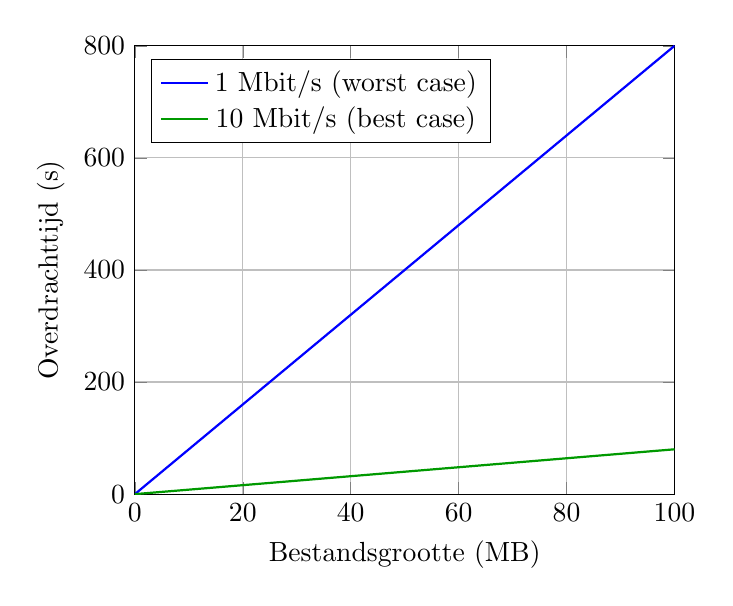
\begin{tikzpicture}
    \begin{axis}[
      xlabel={Bestandsgrootte (MB)},
      ylabel={Overdrachttijd (s)},
      xmin=0, xmax=100,
      ymin=0, ymax=800,
      legend pos=north west,
      grid=major
    ]
    \addplot[blue, thick] coordinates {(0,0)(10,80)(25,200)(50,400)(100,800)};
    \addlegendentry{1 Mbit/s (worst case)}
    \addplot[green!60!black, thick] coordinates {(0,0)(10,8)(25,20)(50,40)(100,80)};
    \addlegendentry{10 Mbit/s (best case)}
    \end{axis}
  \end{tikzpicture}
  \caption{Mock-up: verwachte overdrachttijd in functie van bestandsgrootte bij twee bandbreedtescenario's.}
  \label{fig:mock_bandbreedte}
\end{figure}

Een tweede relevante meting betreft de packet loss in functie van de afstand tussen zender en ontvanger. Op basis van de eigenschappen van straalverbindingen wordt verwacht dat het packet loss percentage laag blijft zolang er een vrije zichtlijn aanwezig is, en sterk toeneemt bij obstructies of bij het overschrijden van de maximale operationele afstand \autocite{MicrowavePtP5G}.

% Mock-up grafiek 2: packet loss vs afstand
\begin{figure}[h]
  \centering
  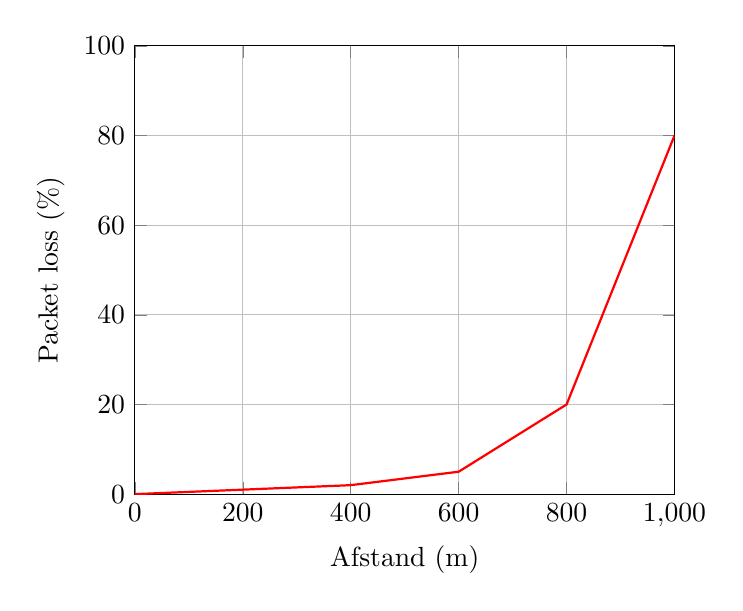
\begin{tikzpicture}
    \begin{axis}[
      xlabel={Afstand (m)},
      ylabel={Packet loss (\%)},
      xmin=0, xmax=1000,
      ymin=0, ymax=100,
      grid=major
    ]
    \addplot[red, thick] coordinates {(0,0)(200,1)(400,2)(600,5)(800,20)(1000,80)};
    \end{axis}
  \end{tikzpicture}
  \caption{Mock-up: verwacht packet loss percentage in functie van de afstand bij een vaste antenneconfiguratie.}
  \label{fig:mock_packetloss}
\end{figure}

\subsection{Meerwaarde voor de doelgroep}

Ongeacht de concrete uitkomst levert dit onderzoek bruikbare informatie op voor IT-professionals en netwerkingenieurs die actief zijn in omgevingen met beperkte connectiviteit. Een werkende proof-of-concept biedt een concreet vertrekpunt voor de uitbouw van robuuste, infrastructuuronafhankelijke bestandstoegangssystemen. Een negatieve uitkomst documenteert de technische grenzen van de huidige aanpak en formuleert aanbevelingen voor alternatieve oplossingsrichtingen. In beide gevallen vult het onderzoek een lacune in de bestaande vakliteratuur, die zich tot op heden niet expliciet heeft gericht op radiogebaseerde toegang tot persoonlijke fileservers.